% Project Improvements remaining
\clearpage%if the chapter heading starts close to bottom of the page, force a line break and remove the vertical vspace
\vspace{21.5pt}
\chapter{Summary}

The project was a success with regard to primary goals, with suitable software solutions to recovering and re-imaging the target board found and implemented to provide a working foundation upon which to build upon, but does not yet provide a full finished package solution.

\section{Improvements and challenges}

Whilst the software functionality attained the planned feature set there still remains hardware interface challenges that need to be solved in order to present a fully deployable solution.

Most notably there still needs to be a quick connection interface designed to allow a target board to be quickly attached to the recovery module. Multiple ways of making this connection have been considered, with the location of the debug points on the two board versions limiting the possibilities notably, especially with the Pico W where they are not located at a castellation point making a fully side mounting clip an impossibility.  The most likely potential method to investigate being some form of mounting clip using pogo pins to make contact with at least the debugging connections, and potentially some form of spring clip or pogo pins for the power supply.

The enable pin could be left off design if power source is under direct control, being which could help simplify design further with only one point outside debug connector needed.

To aid with operation of a clip, the design features a pair of interlock circuit pins that are required to be closed together before power is supplied or enabled to the target board, this is intended to be some form of connection or switch that is activated after the other connections have been made to try and ensure all contacts are closed before any function is performed.

 For simplicity of testing design, this control is currently implemented as controlling the power enable line of the voltage regulator on the target board, but should  be implemented as a MOSFET controlled direct power line or similar so that no power is supplied to the target board till full interlock is achieved, an example proposal of such a driver to control power supply and some simple extra protection resistors added to wiring in \autoref{fig:Wiringwithpowerdriver} using a transistor to drive a P channel MOSFET so that it would be controlled by a high \gls{gpio} signal and thus be in a known state at startup. This would entail some minor code changes to enable power once interlock is closed, but should result in a more robust circuit with lessened risk of wrongly connected pins allowing possible shorts or other unintended behaviour.

\begin{figure}[ht]
	\centering
	\AltText{Proposed extended interconnect design with power driver}{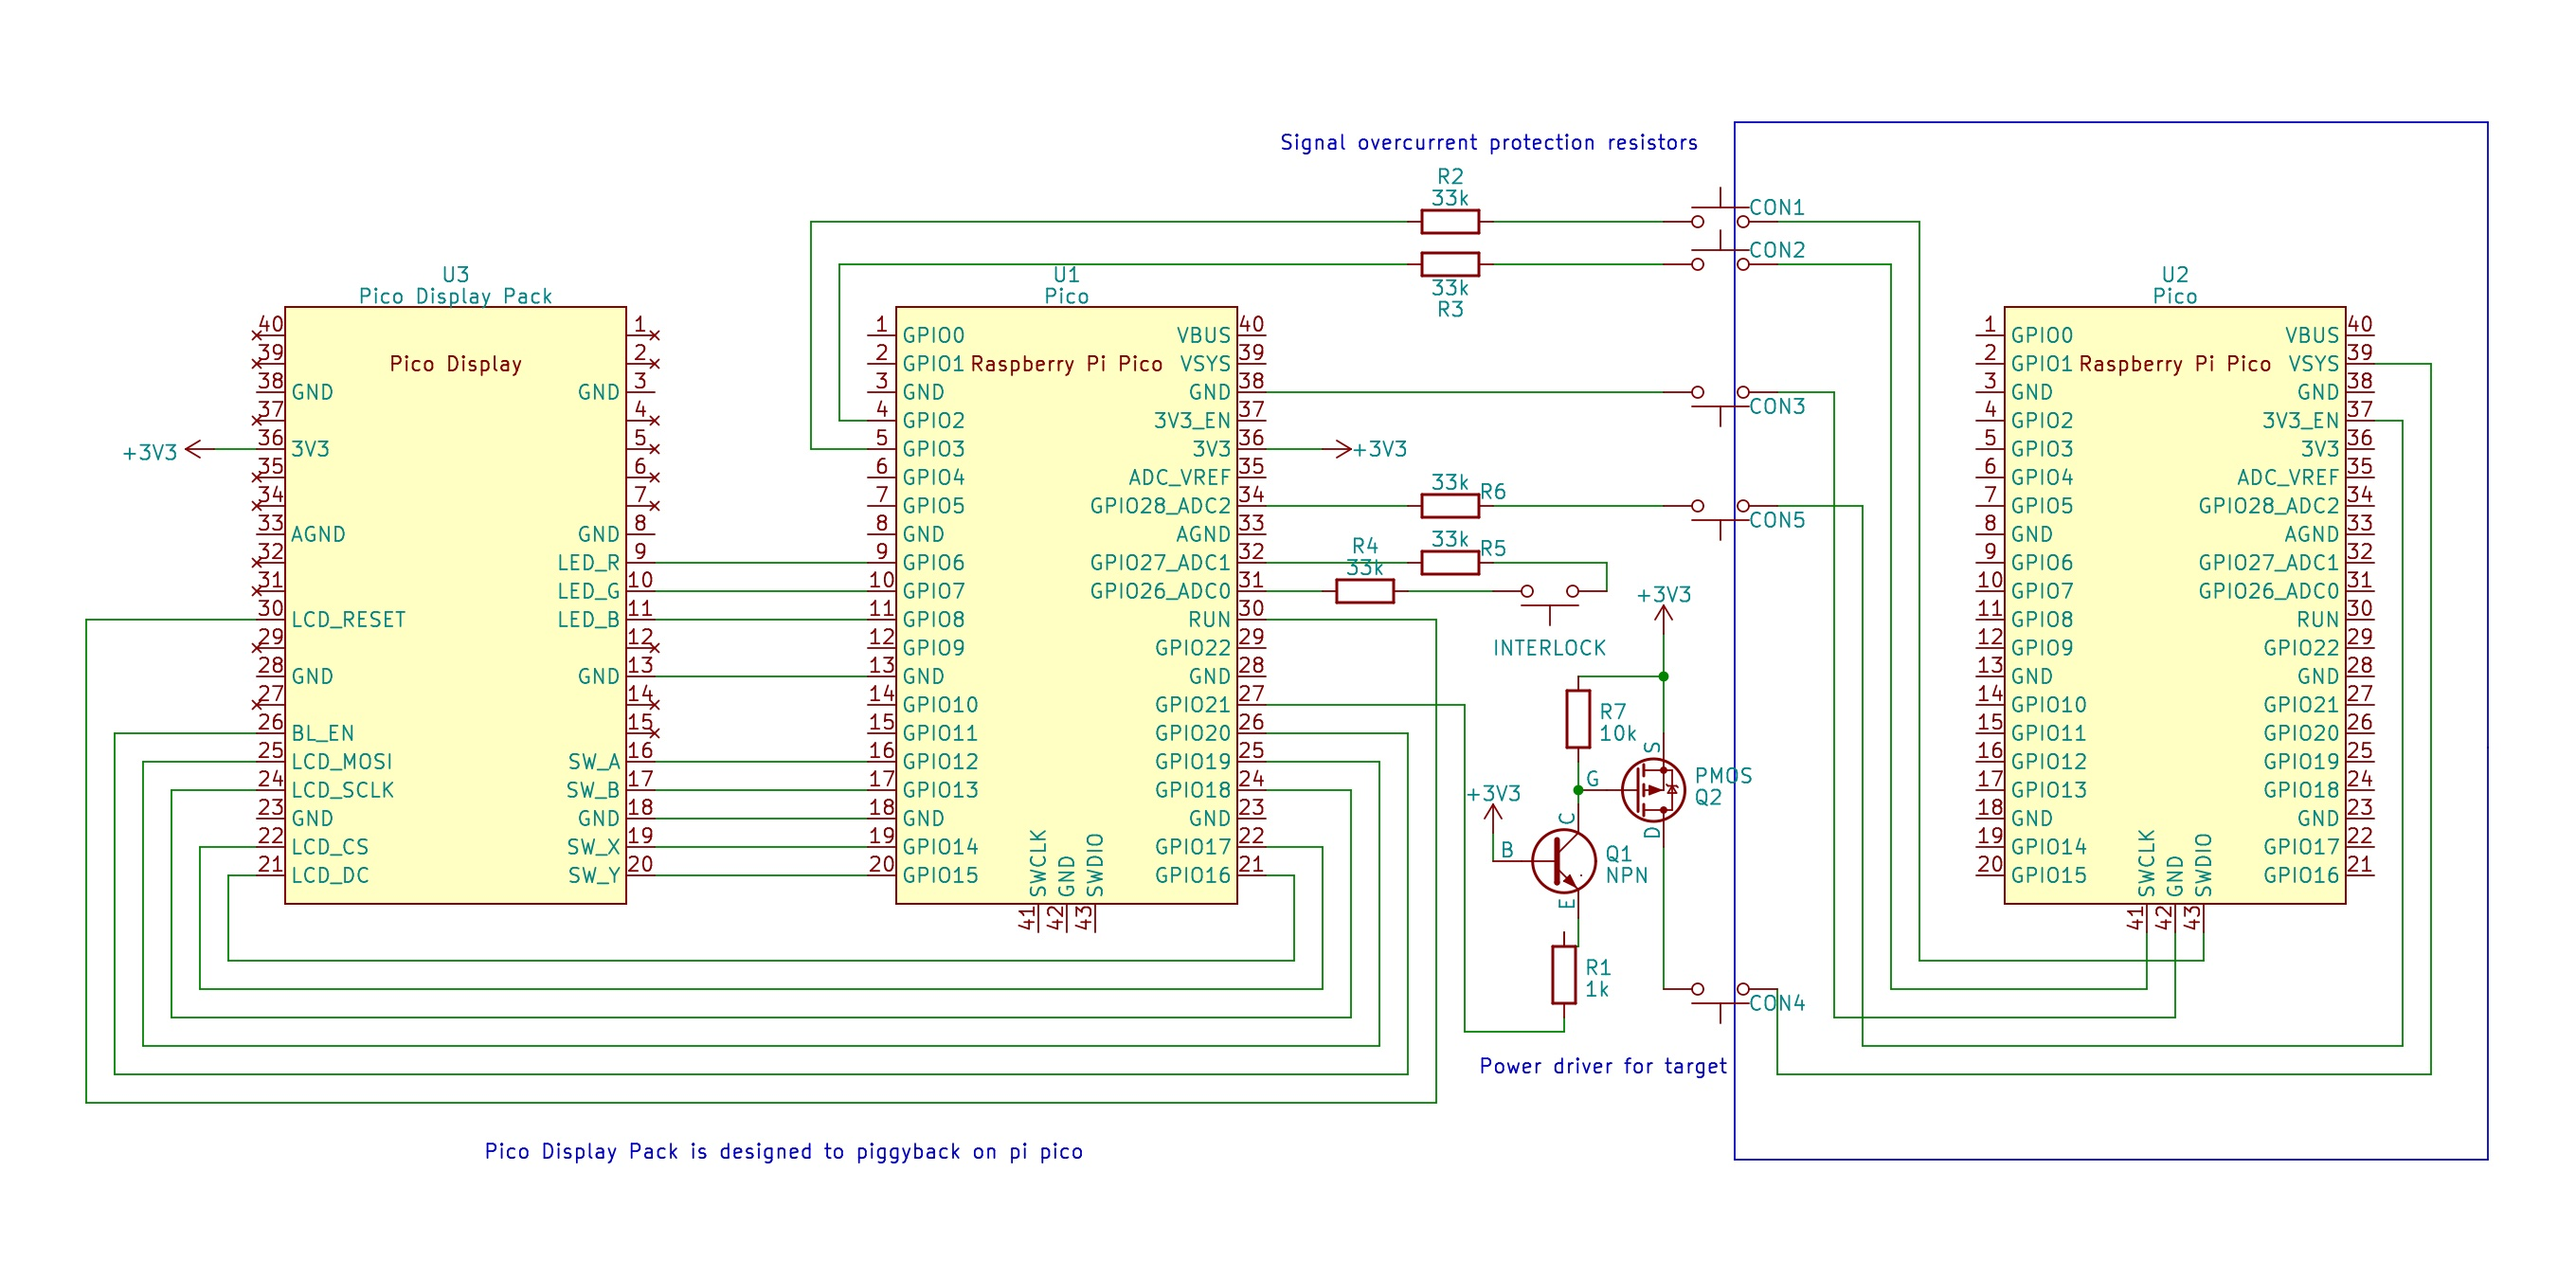
\includegraphics[width=\textwidth]{Schematic with power driver}}
	\caption{Wiring diagram including power driver}
	\label{fig:Wiringwithpowerdriver}
\end{figure}

Due to the test setup another potential is that the reliability of transmission over quick connect contactors has also not been established, which could potentially require more extensive error management. Though due to the relatively slow transmission speeds used in terms of possible \gls{swd} communication frequencies, this is not anticipated to be a major concern, especially for simple recovery procedure where the helper application upload is verified before commencement and retried if necessary already and beyond this communication only involves writing small command packets to memory.

USB connectivity is also notably imperfect presently, especially regarding ejecting and disconnecting/reconnecting USB interface leading to occasional hanging states and need for restarting when connection is started or closed. Though due to updating images being a secondary less commonly performed function of the project, this was deemed to be sufficiently functional for current proof of concept as connection is reliable once established.

Further minor improvements could still be made to file storage, file creation time and date are not presently stored but could be accommodated into storage and file system with minor adjustments.